\documentclass[12pt]{article}
\usepackage{graphicx}
\usepackage{multicol}
\usepackage{fontspec}
\usepackage{xcolor}
\defaultfontfeatures{Mapping=tex-text,Scale=MatchLowercase}
\setmainfont{Open Sans}
\setmonofont{Monaco}[Color=gray]
\title{Intoducing the Best Shared Queue Ever}
%\author{Hossein Naderi}
\date{\today}
\begin{document}
\maketitle

\section{Description of the algorithm}

%In the following sections, we discuss how the abstract version algorithm works and explain its requirements for implementation. The general idea is to have processes agree on the linearization and then respond fast from the history.

\subsection{\texttt{Queue}}
\subsubsection{Definition}
\texttt{Queue} is an ordered set of elements.\subsubsection{Methods}
\paragraph{\texttt{Enqueue(element v)}}
Appends \texttt{v} after the last appended \texttt{element} to the queue.
\paragraph{\texttt{Dequeue()}}
Removes the first not dequeued \texttt{element} in the queue and returns it.
\begin{figure}[hbt]
  \center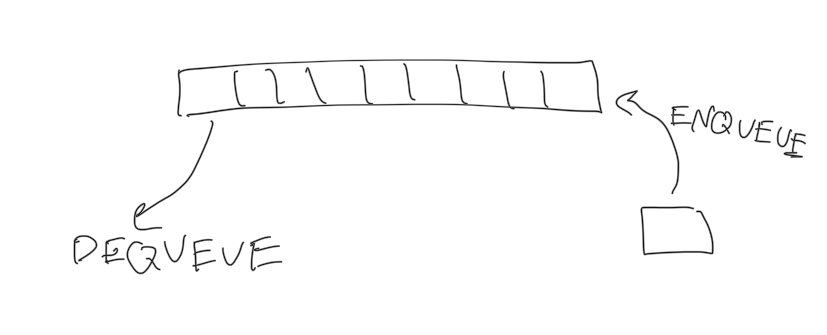
\includegraphics[width=4in]{pics/queue}
  \caption{\texttt{Queue}}
\end{figure}
\subsubsection{Implementation}
 We use a \texttt{Block tree} and a \texttt{Queue helper} implement a \texttt{Queue}. To do an enqueue, it is sufficient to append an enqueue operation to the block tree. For dequeues, we do the same but at last, compute the head using \texttt{Queue helper}, and if the queue is not empty, we return the corresponding enqueue argument.
\subsubsection{Complexity} \texttt{Enqueue(v)} and \texttt{Dequeue()} each take O(log Q+log$^{2}$p) steps.


\subsection{\texttt{‌Block tree}}
\subsubsection{Definition}
\texttt{Block tree} is a data structure that linearizes invocations of \texttt{operation}s by some procesess. \paragraph{Linearization} Operations are linearized when they are added to the root. The operations in a root block are linearized as the block's ordering.
\texttt{TODO}{problem: where should we define the linearization ordering?}
\subsubsection{Methods}
\paragraph{\texttt{Append(operation op)}}
Appends op to the linearization.
\paragraph{\texttt{Get(int i)}}
Returns ith linearized operation.
\paragraph{\texttt{Index(operation op)}}
If Append(op) is terminated, Index(op) returns the order of op in the linearization.
\paragraph{\texttt{Mark(int i)}} If operation i is marked Get(i) is not going to be invoked in future anymore.
\subsubsection{Implementation}
\begin{figure}[hbt]
  \center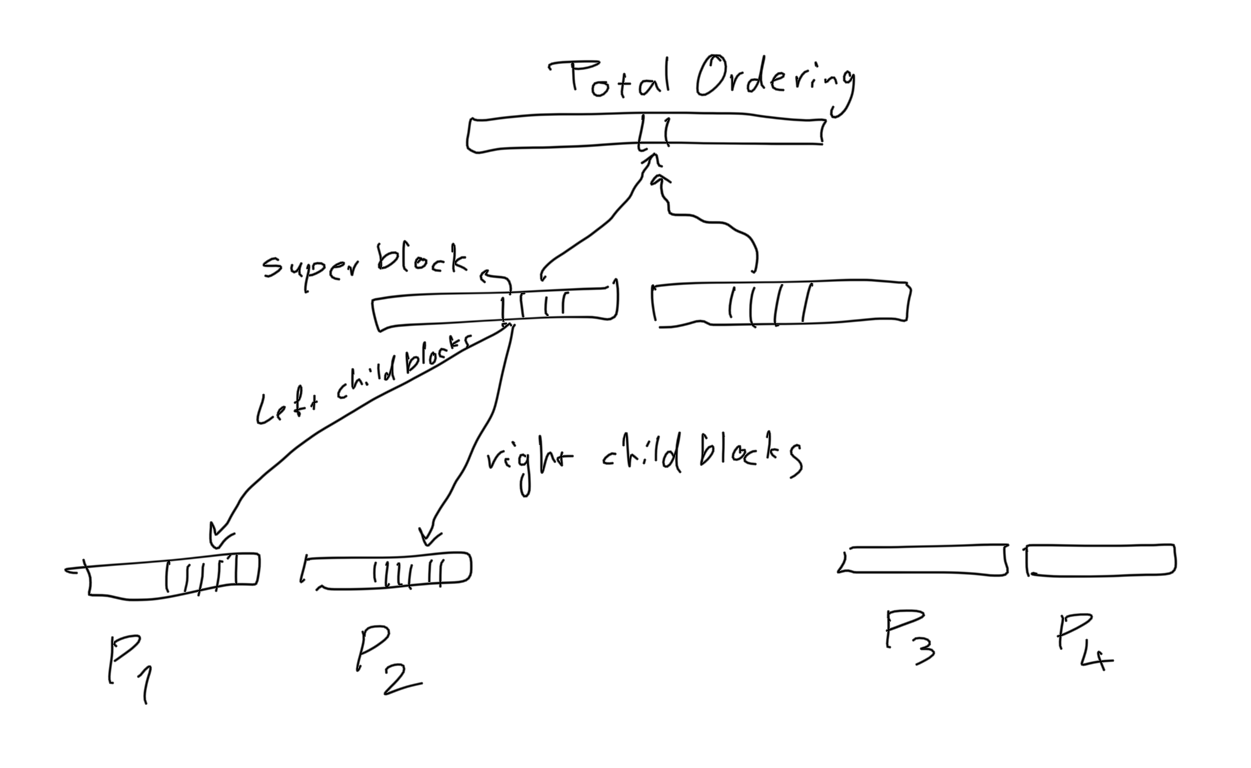
\includegraphics[width=4in]{pics/tree}
  \caption{\texttt{Block tree}}
\end{figure}
\texttt{‌Block tree} is a binary tree of \texttt{node}s, such that a leaf is assigned to each process. Process \texttt{p} adds \texttt{op} to its leaf and propagates it to the \texttt{root node}, which stores the total ordering.
\paragraph{\texttt{Append(op)}}
Adds a block for op to the invoking process's leaf.
\paragraph{\texttt{Propagate(node n)}}
When \texttt{Propagate(node n)} is terminated, operations in n before calling \texttt{Propagate(node n)} are in the root.
\begin{enumerate}
  \item Refresh(n)
  \item If 1 was unsuccessful, do Refresh(n) one more time.
  \item Propagate(n.parent)
\end{enumerate}
\paragraph{\texttt{Get(i)}}
\begin{enumerate}
  \item B= find the root block of containing $i$th op
  \item Get(B, i-pre(B), root)
\end{enumerate}
\texttt{pre(B)} is the number of operations before block B in B's node.
\paragraph{\texttt{Index(op)}}
\begin{enumerate}
  \item B= the block in a leaf containing operation op
  \item Index(n,B,i+pre(B))
\end{enumerate}
\paragraph{\texttt{Mark(i)}} Mark i in the root node.
\subsubsection{Complexity}
\texttt{Append(op)}, \texttt{Get(i)} and \texttt{Index(op)} each take O(log$^{2}$p),
O(log (n-\#marked)+log$^{2}$p),
O(log$^{2}$p) steps.


\subsection{\texttt{Queue helper}}
\subsubsection{Definition}
Queue helper tells us the head of the queue at the time some dequeue operation has been linearized.
\subsubsection{Methods}
\paragraph{\texttt{ComputeHead(i)}} Computes head of the queue when ith dequeue occurs.
\paragraph{\texttt{Augment(i)}} Augments root block i.
\subsubsection{Implementation}
By adding the size and number of non-null dequeues in a block, we can compute the head in constant time.
\subsubsection{Complexity}
Constant time.


\subsection{\texttt{Node}}
\subsubsection{Definition}
A \texttt{node} contains the ordering of the blocks appended to it by time.
\subsubsection{Methods}
\paragraph{\texttt{Append(Block b)}}
Adds \texttt{block b} to the end of the \texttt{node}'s ordering.
\paragraph{\texttt{GetHead()}} Returns the index of the last block added.
\paragraph{\texttt{Refresh(Node n)}}
Creates a block from \texttt{n}'s children's blocks which are not already in \texttt{n}, and tries to append it to \texttt{n}.
\paragraph{\texttt{Get(B,i,n)}} Returns the $i$th operation in block B in node n.
\paragraph{\texttt{Index(n,B,i)}} Returns the superblock in n.parent containing block B in node n.
\subsubsection{Implementation}
\begin{figure}[hbt]
  \center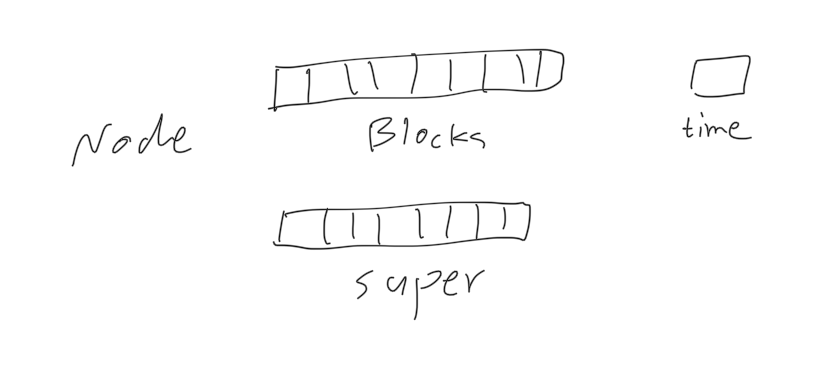
\includegraphics[width=4in]{pics/node}
  \caption{\texttt{Node}}
\end{figure}
\texttt{blocks[i]} stores the ith block. \texttt{time} shows the number of groups propagated to the parent. \texttt{super[i]} is the index of the superblock of the group i.
\paragraph{\texttt{Append(Block b)}} \texttt{CAS}es b to the first empty cell in A.
\paragraph{\texttt{GetHead()}} Returns the head field, it is updated every successful Refresh().
\paragraph{\texttt{Get(B,i,n)}}
\begin{enumerate}
  \item $SB$= find the subblock of B containing $i$th op
  \item Get(SB, i-pre(SB), B's node)
\end{enumerate}
\paragraph{\texttt{Index(n,B,i)}}
\begin{enumerate}
  \item $SB$= find the block in n's parent that contains ith op in block B of node n
  \item Index(n,B,i+pre(SB))
\end{enumerate}
\paragraph{\texttt{Refresh()}}
\begin{enumerate}
  \item Create a block from $n$'s children's blocks which are not already in $n$
  \item Append the block to $n$
  \item If 2 was successful, update the head field
\end{enumerate}
\subsubsection{Requirements} If Append() fails it means another successful instance of Append exists that has some time in common.
\subsubsection{Complexity} Each level of Get() takes $\log p$ steps, and there are $\log p$ levels. So Get may take O(log$^2$ p) steps. Complexity of finding the superblock of a block is O(log p).

\subsection{\texttt{Root node}}
A data structure that contains an ordering of not-marked blocks appended to it.
\paragraph{\texttt{Append(Block b)}}
Adds \texttt{block b} to the end of the \texttt{Root node}'s ordering.
\paragraph{\texttt{Mark(Block b)}}
Marks block b.
\paragraph{\texttt{Get(i)}}
Returns the block containing ith operation.



\subsection{\texttt{Block}}
\subsubsection{Definition}
A block is an ordering of some operations in a node. We can merge some blocks into a block, the initial blocks are called subblocks, and the latter is called superblock.

\texttt{TODO} {problem: where should we put end pointer of blocks that help get become faster?}
\subsubsection{Methods}
\paragraph{\texttt{CreateBlock(operation op)}}
Returns a \texttt{block} that contains \texttt{op}.
\paragraph{\texttt{CreateBlock(node n, int start, int last)}}
Returns a \texttt{block} that contains the blocks from n.start to n.last. The order of the input blocks remains the same.
\paragraph{\texttt{GetEnd()}}
Returns the last left and right subblock of the block.
\subsubsection{Implementation}
\begin{figure}[hbt]
  \center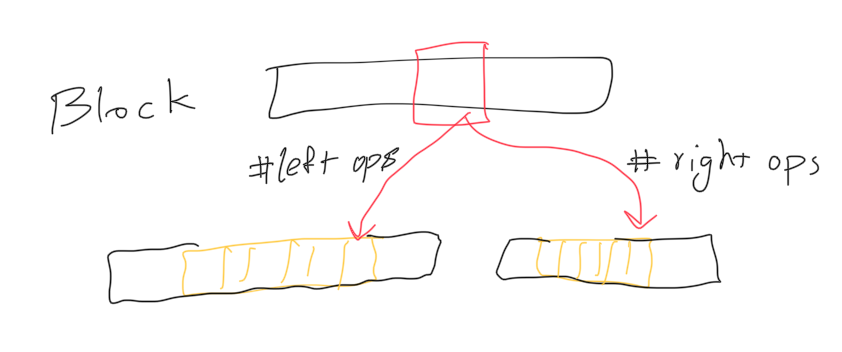
\includegraphics[width=4in]{pics/block}
  \caption{\texttt{Block}}
\end{figure}
We can do the told before methods on blocks only by knowing
\begin{multicols}{2}
\begin{enumerate}
\item \#enqueue operation from left
\item \#enqueue operation from right
\item \#dequeue operation from left
\item \#dequeue operation from right
\item index of the last block from left
\item index of the last block from left
\item group number which tells the blocks which have propagated to the parent together
\end{enumerate}
\end{multicols}
\texttt{TODO} {problem: how to explain the separation of the enqueues from the dequeues? till now, we considered all operations from just one type}

\subsection{\texttt{Operation}}
\subsubsection{Implementation}
Each operation contains the arguments of the operation, the invoking process, and the position in the invoking's process operations.

\end{document}